\chapter{Base de données : OncoPET\_Respi}
	\label{lab:bdd}

\section{Présentation}

Pour répondre à notre problématique de détection des lésions sur les images TEP respirantes, nous avons choisi d’utiliser une base de données d’images simulées. En effet, notre problématique repose sur une connaissance très précise de la position des lésions pour l’évaluation des performances, ainsi que sur l’acquisition de données en mode séquence. Ces deux objectifs sont relativement difficiles à réaliser à partir d’images cliniques, notamment parce que l'acquisition en mode séquence ne fait pas partie de la routine clinique en oncologie.



	\subsection{Avantages des bases de données simulées}

Le principal avantage des bases de données simulées est le contrôle qu'elles permettent d'exercer sur les modèles. Il est possible de spécifier les conditions des acquisitions de manière très précise, et de garantir une homogénéité difficile à atteindre en utilisant des données patient.

Dans le cadre de nos travaux sur la détection, la vérité terrain est particulièrement appréciable, car elle permet de savoir, avec une certitude impossible à atteindre en clinique, la position, le contraste et le nombre des lésions. En effet, dans le cas de lésions de petit diamètre et de petit contraste, le diagnostic ne peut être donné avec une précision totale par le praticien. 

De plus, les simulations permettent d’obtenir des images avec des paramètres qui ne sont pas forcément disponibles en routine clinique. Dans notre cas, la génération des images en mode séquence est indispensable, et très peu d’examens sont réalisés de cette façon, notamment à cause de l’espace disque nécessaire et des temps de reconstruction qu'ils impliquent.

	\section{Modèles}

\subsection{Modèle anatomique}

Nous avons utilisé une base de données d’images TDM fournie par le Centre Hospitalier Lyon-Sud (CHLS) pour créer 15 modèles de patients. Le fantôme paramétrique XCAT~\cite{segars2009mcatoverview} développé par Paul Segars a été déformé de manière manuelle sur chacune des images TDM à l’aide d’un logiciel fourni avec le modèle, présenté dans la figure~\ref{fig:fitXCAT}. Ce modèle est basé sur des surfaces paramétriques NURB (Non-Uniform Rational B-Splines) que l'on peut ajuster manuellement sur les organes d'intérêt du patient en déplaçant les points de contrôle. L'adaptation n’est pas parfaite, du fait des limitations du logiciel, mais permet d’obtenir une variabilité suffisante pour notre étude. Deux images TDM associées aux fantômes adaptés sont présentées dans la figure~\ref{fig:adaptXCAT}.

\begin{figure}
 \centering
 \includegraphics[width=10cm]{images/FIT_XCAT}
 \caption[Adaptation du modèle XCAT sur une image TDM de patient]{Adaptation du modèle XCAT sur une image TDM de patient : le logiciel ne gère pas correctement l'anisotropie des voxels, ce qui explique la déformation du modèle sur la vue de droite. Chaque organe est représenté par une surface paramétrique qu’il est possible d’adapter sur un modèle de patient.}
 \label{fig:fitXCAT}
\end{figure}

Nous avons choisi le XCAT car il intègre directement un modèle de mouvement respiratoire, et il est conçu pour pouvoir être déformé et ainsi engendrer différents patients virtuels.

\begin{figure}
 \centering
 \begin{tabular}{c c}
 \includegraphics[width=4cm]{images/adapt_bru_jea} &
 \includegraphics[width=4cm]{images/adapt_cha_chr}
 \end{tabular}
 \caption[Exemple d’adaptation d’images du modèle XCAT sur des images TDM]{ Exemple d’adaptation d’images du modèle XCAT sur des images TDM : deux modèles XCAT représentés en niveaux de rouge sont adaptés sur des images TDM représentées en vert.}
 \label{fig:adaptXCAT}
\end{figure}


\subsection{Activités des organes}

Les activités des organes sont décrites dans la table \ref{tab:contrastePoumonFoieRecap}. Elles ont été estimées à partir d'une étude réalisée précédemment lors des travaux de thèse de Sandrine Tomeï~\cite{tomei2008development}, en mesurant l'activité dans des zones d'intérêt tracées dans une série de 70 patients~\cite{tomei2010oncopet_db}.

\begin{table}
\centering
 \begin{tabular}{|c|c|c|} 
\hline
Organe 		& Activité ($Bq/cm^3$) \\
\hline
\hline
Foie		& 7740		       \\
\hline
Myocarde	& 11610		       \\
\hline
Os		& 3863		       \\
\hline
Poumon 		& 1338 		       \\
\hline
Prostate	& 2575		       \\
\hline
Rate		& 4939		       \\
\hline
Reins		& 8220		       \\
\hline
Sang		& 5340		       \\
\hline
Tissus mous 	& 2575 		       \\
\hline
Urètre		& 33815		       \\
\hline
Vésicule bilaire& 2575		       \\
\hline
Vessie		& 50973		       \\
\hline
 \end{tabular}

\caption[Activités des organes des patients de la base de données]{Activités définies pour les organes des patients virtuels.}
\label{tab:activiteOrganes}
\end{table}

\subsection{Modèle de Respiration}


Pour prendre en compte la variabilité du cycle respiratoire (voir figure \ref{fig:variabCycle}), nous avons utilisé 4 cycles différents pour modéliser la respiration du patient. Un signal respiratoire complet a été acquis sur une durée de plusieurs minutes à l'aide d'un spiromètre (voir chapitre \ref{lab:spirometre}). Nous avons extrait 3 cycles semblables correspondants à la phase de respiration normale, ainsi qu'un cycle ``anormal'' pour prendre en compte les effets d'une respiration irrégulière du patient pendant une partie du cycle.

\begin{figure}
 \centering
 \begin{tabular}{c c}
 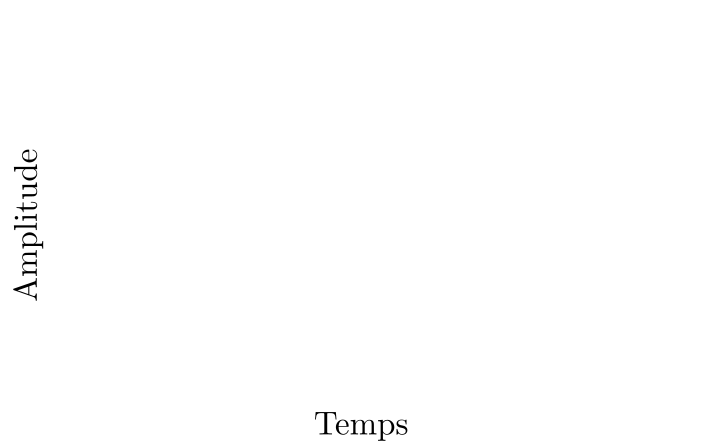
\includegraphics[width=8cm]{images/respiReguliere} &
 \includegraphics[width=8cm]{images/respiIrreguliere}
 \end{tabular}
 \caption[Exemple de courbes respiratoires régulière et irrégulière]{Deux exemples de courbes respiratoires acquises par un spiromètre : celle de gauche montre une respiration régulière, tandis que celle de droite est irrégulière.}
 \label{fig:variabCycle}
\end{figure}


La signal respiratoire obtenu est présenté dans la figure \ref{fig:cycleRespi}. Il est constitué de 4 cycles de 5.6 secondes qui se répètent 10 fois pour former un signal total de 224 secondes, soit un peu moins de 4 minutes. 

Chacun de ces 4 cycles est ensuite discrétisé en 8 parties qui seront utilisées pour générer les modèles de la simulation. 


\begin{figure}
 \centering
 
\includegraphics[width=12cm]{images/courbesRespi}

 \caption[signal respiratoire utilisé pour les modèles de la base de données]{Courbe respiratoire utilisée pour générer les modèles respirants. Les traits verticaux du premier cycle montrent les 8 instants sélectionnés pour discrétiser le mouvement respiratoire de ce cycle.}
 \label{fig:cycleRespi}
\end{figure}

\subsection{Modèle de tumeur}

Nous avons choisi de focaliser cette étude sur la détection des lésions situées dans le foie et les poumons. Ces organes, en effet, sont les plus influencés par le mouvement respiratoire.

Nous avons utilisé un modèle de lésion correspondant adapté aux lésions de faible intensité. Nous avons utilisé des lésions sphériques~\cite{bai2009regularized}, avec des diamètres de l'ordre de la résolution de l'imageur TEP.

Nous avons inséré 280 lésions dans les 15 modèles de patients que nous avons créés. 173 lésions sont présentes dans le poumon, contre 103 dans le foie. La différence de taille entre les organes du XCAT explique la plus petite taille de la base de lésions du foie. 

Les lésions ont été placées manuellement dans tout le volume de l'organe, en privilégiant les parties à fort mouvement proche du diaphragme. 

Les contrastes ont été calibrés pour correspondre à des lésions de faible détectabilité par l'étude suivante :

\subsubsection{Calibration des contrastes des lésions}
\label{lab:etudeDetect}


Notre but est de simuler des images avec un ensemble de tumeurs qui ne soient ni trop évidentes ni impossibles à détecter. Nous avons donc cherché à obtenir une échelle de contrastes qui permette un taux de détection par un observateur humain de 10\%, 30\%, 50\%, 70\% et 90\%.

Pour réaliser cela, un ensemble d'images a été simulé sans mouvement respiratoire, avec différentes tailles de tumeurs et en utilisant, en premier lieu, des valeurs de contrastes présentés dans la base de données créée dans notre laboratoire et présentée dans~\cite{tomei2010oncopet_db}. Les valeurs de contraste de la base OncoPET\_DB sont présentées dans la table~\ref{fig:contrtasteFoiePoumonOrig} pour les lésions du poumon et du foie.


Ensuite, une étude ROC avec deux observateurs humains non médecin a été réalisée afin d'estimer la détectabilité de ces couples activité/taille de tumeurs (fig.\ref{fig:calibration}). 


\begin{table}
\centering
Poumon :\\
\begin{tabular}{|c||c|c|c|c|c|}
 \hline
Poumon	& 10\% & 30\% & 50\% & 70\% & 90\% \\
\hline
8mm	& 2    &  5   &  8   & 10   & 13   \\
\hline
12mm    & 2    &  5   &  8   & 10   & 13   \\
\hline
16mm    & 2    &  3.5 &  4.5 & 7.5  & 10   \\
\hline
\end{tabular}

\vspace{0.5cm}

Foie :\\
\begin{tabular}{|c||c|c|c|c|c|}
 \hline
Poumon	& 10\% & 30\% & 50\% & 70\% & 90\% \\
\hline
8mm	& 2.5    &  4   &  4.5   & 6   & 9   \\
\hline
12mm    & 2    &  3   &  4   & 4.5   & 7.5   \\
\hline
16mm    & 2    &  3   &  4   & 4.5   & 7.5   \\
\hline
\end{tabular}
\caption[Contraste de la base originale OncoPET\_DB des lésions du poumon et du foie pour l'étude de détectabilité]{Contraste de la base originale OncoPET\_DB des lésions du poumon et du foie, avec les pourcentages de détection associés.}
\label{fig:contrtasteFoiePoumonOrig}
\end{table}


On présente à chaque observateur les images les unes après les autres. Ils les annotent en recherchant toutes les lésions et en leur attribuant une note à l'aide du logiciel Amide~\cite{loening2003amide}. La localisation des lésions n'est pas connue à l'avance, et ils doivent donner pour chaque lésion une note entre 1 et 5 correspondant au barème suivant :

\begin{enumerate}
\item Possible.
\item Probable.
\item Très probable.
\item Pratiquement certain.
\item Certain.
\end{enumerate}

Nous avons simulé 5 réalisations d'un même modèle basé sur le XCAT avec 12 lésions différentes implantées dans les poumons et le foie de chaque réalisation. Les données ont été reconstruites avec l'algorithme OPL-EM présenté dans le chapitre~\ref{lab:OPLEM} en utilisant 10 itérations et un seul sous-ensemble. Le choix de ces paramètres a été fixé \textit{a priori} car cette étude est antérieure à la recherche des meilleurs paramètres présentés dans le chapitre 12.

Les résultats de cette étude sont reportés sur les figures~\ref{fig:calibration} et~\ref{fig:calibrationFoie}, qui représentent respectivement le taux de détection des lésions du foie et du poumon moyennée sur 2 observateurs en fonction du contraste.

%Lors de cette étude, nous avons observé que les lésions de la base de données étaient beaucoup trop visibles, ce qui nous a amené à redéfinir les contrastes. 



\begin{figure}[h!]
\centering
\includegraphics[width=16cm]{images/calibration_crop}
\caption[Détectabilité des tumeurs du poumon en fonction du contraste et de la taille des tumeurs]{Détectabilité des tumeurs du poumon moyennée sur 2 observateurs en fonction du contraste et de la taille des tumeurs. Chaque courbe représente une taille de lésion différente.} 
\label{fig:calibration}
\end{figure}

\begin{figure}[h!]
\centering
\includegraphics[width=16cm]{images/calibrationFoie_crop}
\caption[Détectabilité des tumeurs du foie en fonction du contraste et de la taille des tumeurs]{Détectabilité des tumeurs du foie moyennée sur 2 observateurs en fonction du contraste et de la taille des tumeurs. Chaque courbe représente une taille de lésion différente.} 
\label{fig:calibrationFoie}
\end{figure}


\begin{table}
\centering
Poumon :\\
\begin{tabular}{|c|c|c|c|}
 \hline
 Détection voulue & 	8mm & 	12mm & 	16mm \\
\hline
90 \%		  & 100 \%  & 100 \% & 100 \% \\
\hline
70 \%		  & 100 \%  & 100 \% & 90 \%\\
\hline
50 \%		  & 90 \%  & 100 \% & 100 \%\\
\hline
30 \%		  & 44 \%  & 90 \% & 30 \%\\
\hline
10 \% 		  & 0 \%  & 0 \% & 0 \%\\
\hline
\end{tabular}

\vspace{0.5cm}

Foie :\\
\begin{tabular}{|c|c|c|c|}
 \hline
 Détection voulue & 	8mm & 	12mm & 	16mm \\
\hline
90 \%		  & 100 \%  & 100 \% & 100 \% \\
\hline
70 \%		  & 100 \%  & 75 \% & 100 \%\\
\hline
50 \%		  & 85 \%  & 100 \% & 75 \%\\
\hline
30 \%		  & 100 \%  & 100 \% & 100 \%\\
\hline
10 \% 		  & 30 \%  & 75 \% & 90 \%\\
\hline
\end{tabular}
\caption[Détectabilité estimée des lésions en fonction du contraste et de leur diamètre]{Détectabilité des lésions réalisée à l'aide d'une étude par des humains sur 5 patients totalisant 60 lésions. La colonne de gauche indique la détectabilité des lésions calibrée pour OncoPET\_BD.}
\label{fig:detectabiliteVue}
\end{table}

Ces résultats sont également résumés dans la table~\ref{fig:detectabiliteVue}. Ils montrent une détectabilité largement supérieure à celle que nous avions estimée initialement à partir des résultats obtenus sur la première base de données OncoPET\_DB. Les écarts peuvent s'expliquer par le fait que nous n'avons pas simulé le même scanner TEP (Caméra HR+ pour la base OncoPET\_BD, Philips Gemini pour la nouvelle base), et que les données ont été reconstruites avec un algorithme différent. Il s'avère également que les lésions de 16 mm sont trop visibles pour être intégrées dans l'étude. Nous avons fait des interpolations linéaires entre les statistiques obtenues pour définir les nouvelles gammes d'activités. Les valeurs de contraste utilisées dans notre étude sont finalement reportées dans la table \ref{tab:contrasteFoieFinal} pour les lésions du foie et du poumon.



\begin{table}

\centering

\begin{tabular}{|c||c|c||c|c|}
 \hline
	& 8mm Foie	& 12mm Foie	& 8mm Poumon	& 12mm Poumon	\\
\hline
10\%	& 1.8		& 1.3		& 3.0		& 2.5		\\
\hline
30\%	& 2.0		& 1.5		& 4.0		& 3.0		\\
\hline
50\%	& 2.5		& 1.8		& 5.0		& 3.5		\\
\hline
70\%	& 3.0		& 2.0		& 6.5		& 4.0		\\
\hline
90\%	& 3.5		& 2.3		& 8.0		& 5.0		\\
\hline
\end{tabular}
\caption[Contraste final lésions du foie et du poumon]{Contrastes appliqués aux lésions de la base de données en fonction du taux de détectabilité désiré.}
\label{tab:contrasteFoieFinal}
\end{table}

\section{Simulation}

Nous avons utilisé le logiciel SORTEO pour simuler la caméra TEP de l'imageur TEP/TDM Philips Gemini. La simulation a été réalisée sur 3 lits, avec un recouvrement de 9 cm par lits. Pour référence, le champ de vue axial de l'imageur est de 18 cm.

Nous avons réalisé les simulations de deux acquisitions :
\begin{description}
\item[Dynamique :] Les 8 modèles de chacun des 4 cycles respiratoires ont été simulés séparément pour chaque lit. La durée de chaque examen simulé est de 7 secondes, ce qui représente une simulation totale de 224 secondes. Les données simulées de chaque cycle sont concaténées pour simuler le résultat d'une acquisition avec synchronisation respiratoire, et former 8 fichiers de données séquence par lit.
\item[Statique :] Le modèle de fin d'expiration a été utilisé pour simuler un examen de 224 secondes par lit pour correspondre à la durée de la simulation dynamique.
\end{description}

Le temps de simulation nécessaire pour générer une image statique est de 110 h par processeur environ, contre 130 heures pour générer une image dynamique. La différence de temps s'explique par le processus de simulation. En effet, chaque simulation est réalisée en deux temps (voir~\ref{lab:simuSORTEO}), dont le premier a une durée fixe, qui est réalisée pour chacune des 8 simulations des 4 cycles dans le cadre de la simulation dynamique, et seulement une fois pour la simulation statique.

Le volume de données généré est d'environ 6 Go par patient sans prendre en compte les données intermédiaires générées lors de la simulation.

\subsection{Exemples de données reconstruites}

La base de données générée contient les données de simulation de 15 patients, reconstruits avec une correction parfaite (image statique), sans correction, et avec deux méthodes de correction du mouvement respiratoire présentées dans les sections \ref{lab:corrPostRecon} et \ref{lab:CorrpendantRecon}. Deux exemples d'images reconstruites complètes sont visibles sur la figure~\ref{fig:exempleImageRecon}. La figure~\ref{fig:exempleImageReconMvt} illustre le mouvement respiratoire dans les images reconstruites.

\begin{figure}
 \centering
 
\includegraphics[width=15cm]{images/exempleImageRecon}
 \caption[Images reconstruites tirées de la base de donnée]{Images reconstruites (8 itérations et 5 sous-ensembles) à partir des simulations de la base de données. Les flèches représentent une lésion du foie de diamètre 8 mm avec un contraste de 3.5 : patient 1, ainsi que deux lésions du poumon de 8 mm et de contraste 6.5 : patient 2.}
 \label{fig:exempleImageRecon}
\end{figure}

\begin{figure}
 \centering
 
\includegraphics[width=14cm]{images/exempleImageReconMouvement}
 \caption[Images respirantes reconstruites tirées de la base de donnée]{Images reconstruites (8 itérations et 5 sous-ensembles) à partir des simulations statiques a) et dynamiques b),c) et d) de la base de données. b), c) et d) représentent respectivement les données du premier instant temporel (fin d'expiration), du troisième et du quatrième. L1 représente une lésion pulmonaire de 8 mm et de contraste 8, L2 une lésion hépatique de 12 mm et de contraste 1.5, L3 et L4 des lésions hépatiques de diamètre 12 mm et de contraste de 2.3.}
 \label{fig:exempleImageReconMvt}
\end{figure}

\section{Données clef} % temps de calculs etc....

Cette section correspond à un résumé des caractéristiques de la base de données.

\subsection{Modèles}

Nous avons créé 15 modèles, qui ont été adaptés depuis autant d'images TDM fournies par le centre hospitalier Lyon-SUD. Pour cela nous avons utilisé les outils fournis par Paul Segars~\cite{segars2001These}.


\subsection{Lésions}

Nous avons inséré 280 lésions dans les 15 modèles de patients que nous avons créés. 173 lésions sont présentes dans le poumon, contre 107 dans le foie. La différence de taille entre les organes explique la plus petite taille de la base de lésions du foie. 

Les lésions ont été placées manuellement dans tout le volume de l'organe, en préférant les parties à fort mouvement proche du diaphragme. 

Le tableau~\ref{tab:contrastePoumonFoieRecap} récapitule les contrastes, ainsi que les tailles des lésions implantées dans les organes.
 
\begin{table}
\centering
 \begin{tabular}{|c|c||c|c|c|c|c|} 
\hline
\multicolumn{2}{|c|}{Niveau de confiance}       & 1	  & 2	    & 3	     & 4	& 5	\\
\hline
\hline
Poumon	(173)	& 8 mm (90)	& 3 (19)  & 4 (18)  & 5 (18)  & 6.5 (18)	& 8 (17)\\
\cline{2-7}
		& 12 mm	(83)	& 2.5 (16)& 3 (16)  & 3.5 (18)& 4 (17)	& 5 (16)\\
\hline
Foie 	(107)	& 8 mm (54)		& 1.8 (11)& 2 (11)  & 2.5 (10)& 3 (11)	& 3.5 (11)\\
\cline{2-7}
		& 12 mm	(53)	& 1.3 (10)& 1.5 (10)& 1.8 (11)& 2 (11)  & 2.3 (11)\\
\hline 
 \end{tabular}

\caption[Tableau récapitulatif des lésions]{Tableau récapitulatif des contrastes des lésions présentes dans le foie et les poumon des modèles. le nombre de lésions est indiqué entre parenthèses.}
\label{tab:contrastePoumonFoieRecap}


\end{table}



